\chapter{Sviluppo ed Utilizzo}
\label{chapter:implementazione}

\section[Sistema Realizzato per Simulazioni ed Analisi]{Sistema Realizzato per Simulazioni ed\\ Analisi}
\label{section:sistema_analisi}

Al fine di valutare le prestazioni degli scenari di Fog Computing, descritti al capitolo \ref{chapter:architettura}, è stato implementato un sistema di simulazione che ne permette in una prima fase la definizione in ogni suo aspetto (topologia, applicazioni, servizi, richieste, ecc...) e, successivamente, l'analisi dei principali aspetti utili alla comprensione dello scenario, come il successo del \textit{service placement} e delle richieste di servizi da parte dei vari nodi della rete.

La definizione e l'esecuzione della simulazione seguono il diagramma di flusso mostrato in Figura \ref{fig:sim_flow_diagram}. Come accennato è possibile eseguire due principali tipologie di analisi:
\begin{enumerate}
	\item \textbf{Analisi del service placement}. È possibile analizzare l'andamento del service placement al variare di specifici parametri di definizione dello scenario, specificando il numero di iterazioni e quali di questi devono variare ad ogni esecuzione.
	\item \textbf{Analisi della simulazione}. Una volta definito e simulato uno specifico scenario, è possibile ottenere un'analisi sul soddisfacimento delle richieste da parte dei nodi dei vari servizi offerti dalla rete, con e senza \textit{failure control} dei nodi/servizi.
\end{enumerate}


\begin{figure}[!ht]
  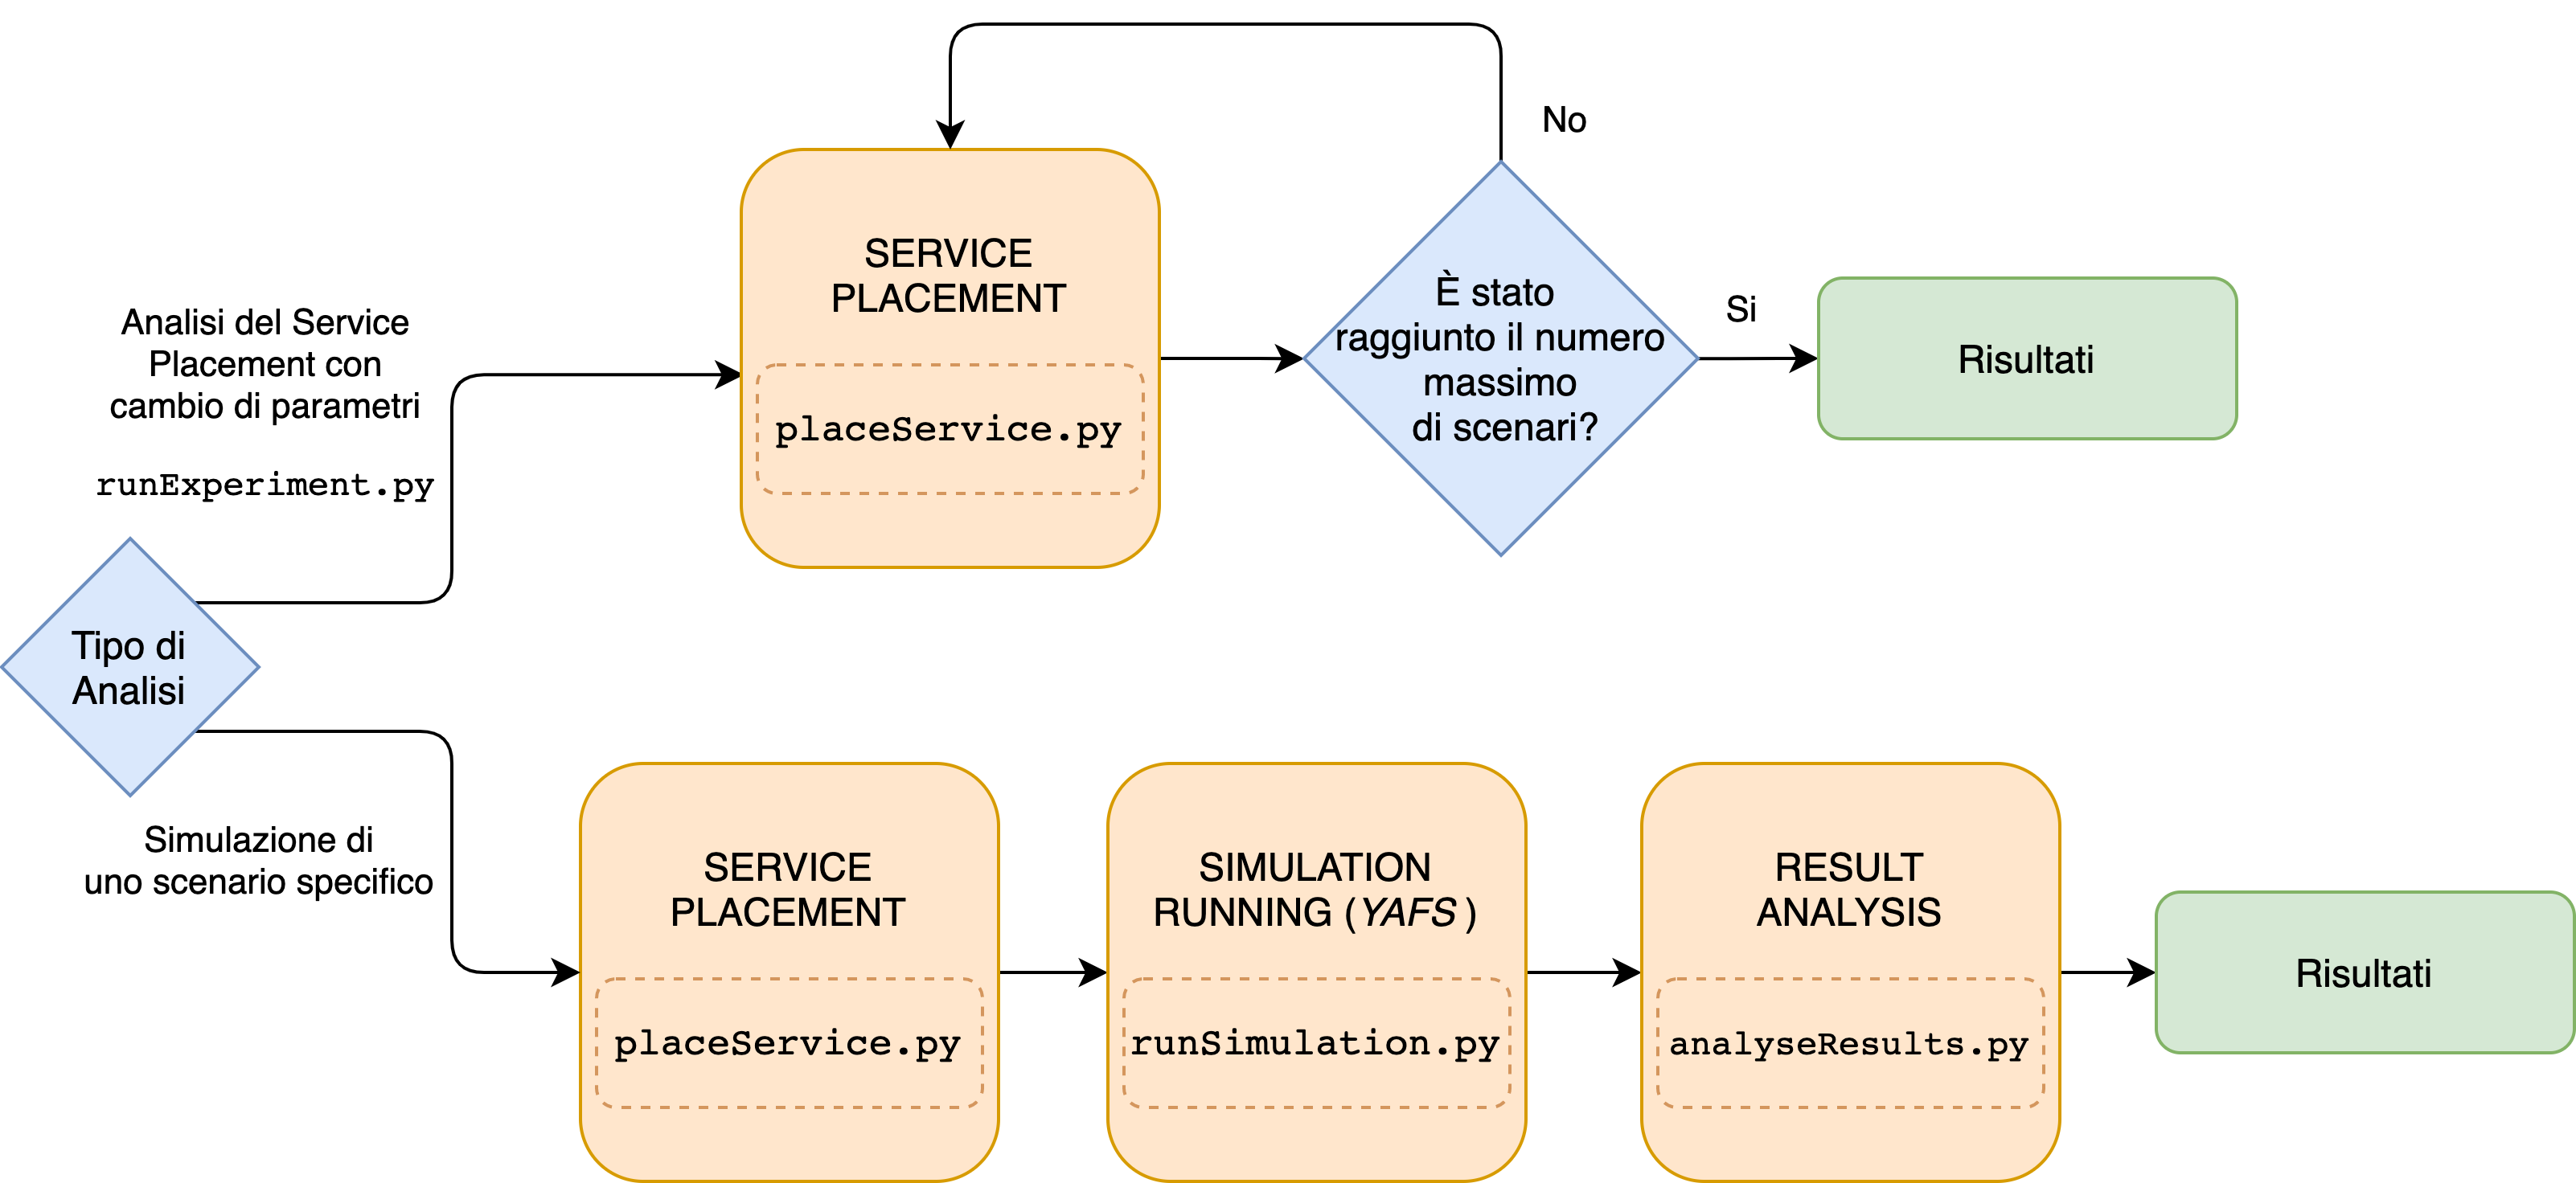
\includegraphics[width=14cm]{images/sim_flow_diagram}
  \centering
  \caption{Diagramma di flusso del sistema di simulazione.}
  \label{fig:sim_flow_diagram}
\end{figure}

\subsection{Utilizzo del Software Realizzato}

% TODO scrivere qui la questione della generazione della topologia, dei dettagli in experiment configuration, la distinzione tra le due vie di simulazione e così via.

\section{Implementazione del Simulatore}

In questo paragrafo verranno approfonditi i singoli aspetti che compongono il processo esposto al Paragrafo \ref{section:sistema_analisi}, nonché il loro utilizzo per la definizione e l'esecuzione delle simulazioni.

\subsection{Algoritmo di Service Placement}

Per ottenere il massimo beneficio dall'implementazione di un'architettura Fog, è necessario un efficace algoritmo di \textit{service placement}. In generale questi algoritmi sono improntati a massimizzare il \textit{Quality of Service}\footnote{Con \textit{Quality of Service} si intende l'insieme dei valori che indicano la qualità del servizio offerto dalla rete, in termini di throughput, gestione degli errori, gestione dei ritardi e utilizzo della banda.} (QoS) o il bilanciamento del carico, oppure a minimizzare il consumo di energia, la latenza o il costo della comunicazione.

In questo lavoro di Tesi, l'algoritmo implementato\footnote{In: \texttt{placeService.py}} è fondato su due aspetti principali: preservare la \textit{privacy} dei dati scambiati tra i servizi e far si che le applicazioni siano disponibili per gli utenti il più velocemente possibile. L'algoritmo utilizza un approccio \textit{Greedy}\footnote{L'approccio \textit{Greedy}, come paradigma negli algoritmi, indica la costruzione della soluzione ottima scegliendo, ad ogni iterazione, la via che offre il maggiore vantaggio in quello specifico stadio. } valutando i diversi aspetti dei servizi, come privacy, risorse necessarie e \textit{deadlines} delle applicazioni. La privacy dei servizi è relativa al loro livello di piazzamento: con livelli di privacy crescenti (la sensibilità dei dati), i servizi potranno essere piazzati solo in livelli via via più bassi, ovvero più vicino al livello IoT. La tendenza dell'algoritmo è quella di allocare le applicazioni il più vicino possibile al livello IoT, così da minimizzare la latenza.

Il primo passo che viene compiuto è l'ordinamento delle applicazioni secondo un ordine crescente sulla base del livello di privacy dei servizi che la compongono. In particolare viene utilizzato il seguente approccio:
\begin{equation*}  
	\begin{array}{c}

\displaystyle \operatorname{privacy}(APP_x) \leq \operatorname{privacy}(APP_y)\\
\text{se e soltanto se}\\
\displaystyle \min_{S_u \in APP_x} \operatorname{privacy}(S_u) \leq \min_{S_v \in APP_y} \operatorname{privacy}(S_v)
 	\end{array}
\end{equation*}
dove $S_u$ e $S_v$ sono i servizi delle singole applicazioni. Nel caso particolare in cui due applicazioni abbiamo lo stesso valore di privacy, allora verranno ordinate secondo la loro \textit{deadline}, in ordine crescente.

Una volta eseguito l'ordinamento delle applicazioni, l'algoritmo di placement comincia ad allocare i servizi iniziando dalla prima applicazione della lista. L'algoritmo tende a posizionare i servizi nei primi nodi disponibili cominciando da quelli più vicini agli utenti (livello IoT). Nel caso di insufficienza di risorse e se il livello di privacy lo permette, i servizi vengono allocati nel Cloud. Una applicazione viene considerata ``allocata" se e solo se lo sono tutti i suoi servizi, altrimenti viene scartata.

Le applicazioni che l'algoritmo di \textit{service placement} tenta di allocare, sono generate nella configurazione dell'esperimento.

\subsection{Experiment Configuration}

La configurazione dell'esperimento\footnote{In: \texttt{config/experimentConfiguration.py}} gestisce la generazione della topologia di rete, delle applicazioni e degli utenti, ovvero i dispositivi che generano le richieste dei servizi.

\subsubsection{Generazione della Topologia}

Come accennato nel capitolo \ref{chapter:architettura}, il simulatore \textit{YAFS} utilizza \textit{NetworkX} come base per l'analisi e l'utilizzo dei grafi. La stessa libreria \textit{python} è stata dunque utilizzata anche per la generazione della rete.

Per semplicità è stato introdotto un livello di \textit{gateway}, il cui scopo è quello di fungere da intermediario da i dispositivi IoT e la rete. I nodi di questo livello sono generati come mostrato di seguito.

\begin{lstlisting}[language=python]
H.add_nodes_from([(i, {"level[z]": level}) for i in range(iot_nodes // 5)])
\end{lstlisting}

La divisione del numero di nodi IoT (\texttt{iot\_nodes}) per 5, indica che il numero dei \textit{gateway} accennati sopra, saranno $1\backslash 5$ del numero di nodi IoT.

Per i livelli successivi viene utilizzato, come descritto nel paragrafo \ref{section:interconnesione_livelli}, il modello \textit{Watts-Strogatz}:
\begin{lstlisting}[language=python]
# Number of nodes of upper levels
new_nodes = iot_nodes // (fogi_reduction_factor ** (level-1)) if iot_nodes // (fogi_reduction_factor**(level-1)) >= 2 else 2
                
# Small-World graph generation for FOG levels greater than 0 (e.g provincial fog nodes)
H = nx.watts_strogatz_graph(int(new_nodes), 2, hub_prob)
\end{lstlisting}




